

In this section, we introduce three graphical models as extensions for
the TrueSkill factor graph (Figure~\ref{fig:trueskill}) to incorporate
score-based outcomes in skill learning.  Our first two graphical
models are motivated by modeling score-based outcomes as generated by
separate offence and defence skills for each team.  The first
generative score model uses a Poisson, which is natural model when
scores are viewed as counts of scoring events.  The second generative
model uses a simpler Gaussian model.  Our third model is a simplified
version of the Gaussian model, which like TrueSkill, only models a
single skill per team (not separate offence/defence skills) and places
a Gaussian likelihood on the score difference, which may be positive
or negative.  Next we formulate each model in detail.

\subsection{Offence and Defence Skill Models}
\label{sec:PoissonGraphicalModel}

In a match between two teams $i$ and $j$ producing respective scores
$s_i \in \mathbb{Z}$ and $s_j \in \mathbb{Z}$ for each team, it is natural to
think of $s_i$ as resulting from $i$'s offence skill $o_i \in \mathbb{R}$
and $j$'s defence skill $d_j \in \mathbb{R}$
(as expressed in any given match) and
likewise for $j$'s score as a result of $j$'s offence skill
$o_j \in \mathbb{R}$
and $i$'s defence skill $d_i \in \mathbb{R}$.  This is contrasted
with the univariate skill estimates of team $i$'s skill $l_i$
and team $j$'s skill $l_j$ used in TrueSkill, which lump together
offence and defence skills for each team.

Given scores $s_i$ and $s_j$ for teams $i$ and $j$, we model the
generation of scores from skills using a conditional probability
$p(s_i, s_j|o_i, o_j, d_i, d_j)$. We assume that team $i$'s score
$s_i$ depends only on $o_i$ and $d_j$ and likewise that team $j$'s
score $s_j$ depends only on $o_j$ and $d_i$:
\begin{align}
  p(s_i, s_j|o_i, o_j, d_i, d_j) = p(s_i|o_i,  d_j)p( s_j|o_j, d_i).
\label{eq:sampleAssumption}
\end{align}
Like TrueSkill, we assume that the joint marginal over skill
priors independently factorises:
\begin{align}
  p(o_i, o_j, d_i, d_j) = p(o_i) p(d_j) p(o_j) p(d_i).
\end{align}
Given an observation of scores $s_i$ for team $i$ and $s_j$ for team
$j$, the problem is to update the posterior distributions over
participating teams' offence and defence skills.  According to
Bayes rule and the previous assumptions, the posterior distribution
over $(o_i, o_j, d_i, d_j)$ is given by
\begin{align}\label{eq:Bay}
    p(o_i, d_i, o_j, d_j | s_i, s_j) & \propto p( s_i, s_j |o_i, d_i, o_j, d_j ) p(o_i, d_i, o_j, d_j) \nonumber \\
        & \propto [p(s_i|o_i,d_j) p(o_i) p(d_j)] \; [p(s_j|o_j,d_i)  p(o_j) p(d_i)].
\end{align}
Here we observe that estimating $p(o_i, d_i, o_j, d_j | s_i, s_j)$
factorises into the two independent inference problems:
\begin{align}
p(o_i, d_j|s_i) & \propto p(s_i|o_i,d_j) p(o_i) p(d_j), \text{and} \\
p(o_j, d_i|s_j) & \propto p(s_j|o_j,d_i) p(o_j) p(d_i).
\end{align}
All models considered in this paper (including TrueSkill) assume
Gaussian priors on team $i$'s offence and
defence skills, i.e., $p(o_i):=\mathcal{N}(o_i; \mu_{oi}, \sigma_{oi}^2)$
and $p(d_i):=\mathcal{N}(d_i; \mu_{di}, \sigma_{di}^2)$.  Our objective
then is to estimate the means and variances for the posterior distributions
of $p(o_i, d_j|s_i)$ and $p( o_j, d_i |s_j)$.  So far, the only missing pieces
in this skill posterior update are the likelihoods $p(s_i|o_i,d_j)$
and $p(s_j|o_j,d_i)$ that specify how team $i$ and $j$'s offence and
defence skills probabilistically generate observed scores.  For this
we discuss two possible models in the following subsections.

\subsubsection{Poisson Offence/Defence Skill Model}

Following TrueSkill, we model the generation of match outcomes
(in our case, team scores) based on stochastic offence and defence
\emph{performances} that account for day-to-day performance
fluctuations. Formally, we assume that team $i$ exhibits offence performance
$p_{oi}:=\mathcal{N}(p_{oi}; o_i, \beta_o^2)$ and defence performance
$p_{di}:=\mathcal{N}(p_{di}; d_i, \beta_d^2)$. With these
performances, we model team $i$'s score $s_i$ as generated from the
following process: team $i$'s offence performance $p_{oi}$ promotes
the scoring rate while the defence performance $p_{dj}$ inhibits this
scoring rate, the difference $p_{oi}-p_{dj}$ being the effective
scoring rate of the offence against the defence.

Finally, we model the score by $s_{i}\sim\text{Poisson}(\lambda)$,
where a requirement of a positive rate $\lambda$ for the Poisson distribution
requires the use of $\lambda = \exp(p_{oi}-p_{dj})$ since
$p_{oi}-p_{dj}$ may be negative.\footnote{This exponentiation of
$p_{oi}-p_{dj}$ may seem to be made only to ensure model correctness,
but we show experimentally that it has the benefit of
allowing the Poisson model to accurately predict scores in
high-scoring games even when team skills are very close (and hence
$p_{oi}-p_{dj} \approx 0$).}  Likewise, one can model $s_j$ by
applying the same strategy when given $\lambda = \exp(p_{oj} - p_{di})$.
We represent the resulting \emph{Poisson-OD}
model in Figure~\ref{fig:trueskill_variant} where the joint posterior
is
\begin{align}%\label{eq:BayTransNew2}
    p(o_i, d_j, p_{oi},p_{dj} | s_i) & \propto p(s_i|p_{oi},p_{dj}) p(p_{oi}|o_i) p(p_{dj}|d_j) p(o_i)p(d_j), \nonumber \\
    p(o_j, d_i, p_{oj},p_{di} | s_j) & \propto p(s_j|p_{oj},p_{di}) p(p_{oj}|o_j) p(p_{di}|d_i) p(o_j)p(d_i). \nonumber
\end{align}
We are only interested in the posterior distributions of $o_i,d_j$ and
$o_j,d_i$ given $s_i$ and $s_j$, respectively. Thus, we integrate
out the latent performance variables to obtain the desired posteriors
\begin{align} %\label{eq:BayTransNew3}
    p(o_i, d_j | s_i) &= \int_{-\infty}^{+\infty} \int_{-\infty}^{+\infty} p(o_i, d_j, p_{oi},p_{dj} | s_i)  \mathrm{d}p_{oi}\mathrm{d}p_{dj}, \nonumber \\
    p(o_j, d_i | s_j) &= \int_{-\infty}^{+\infty} \int_{-\infty}^{+\infty} p(o_j, d_i, p_{oj},p_{di} | s_j)  \mathrm{d}p_{oj}\mathrm{d}p_{di}. \nonumber
\end{align}
\unindentmore Like TrueSkill, we use Bayesian updating to update beliefs in the
skill levels of both teams in a pairwise match based on the score
outcome, thus leading to an online learning scheme.  Posterior
distributions are approximated to be Gaussian and used as the
priors in order to learn each team's skill for the next match.
Approximate belief updates via variational Bayesian inference in this model
will be covered in Section~\ref{sec:PoissonInference}.
%
%%%%%%%%%%%%%%%%%%%%%%%%%%%%%%%%%%%%%%%%%%%%%%%%%%%%%%%%%%%%%%
\begin{figure}[t!]
\centerline{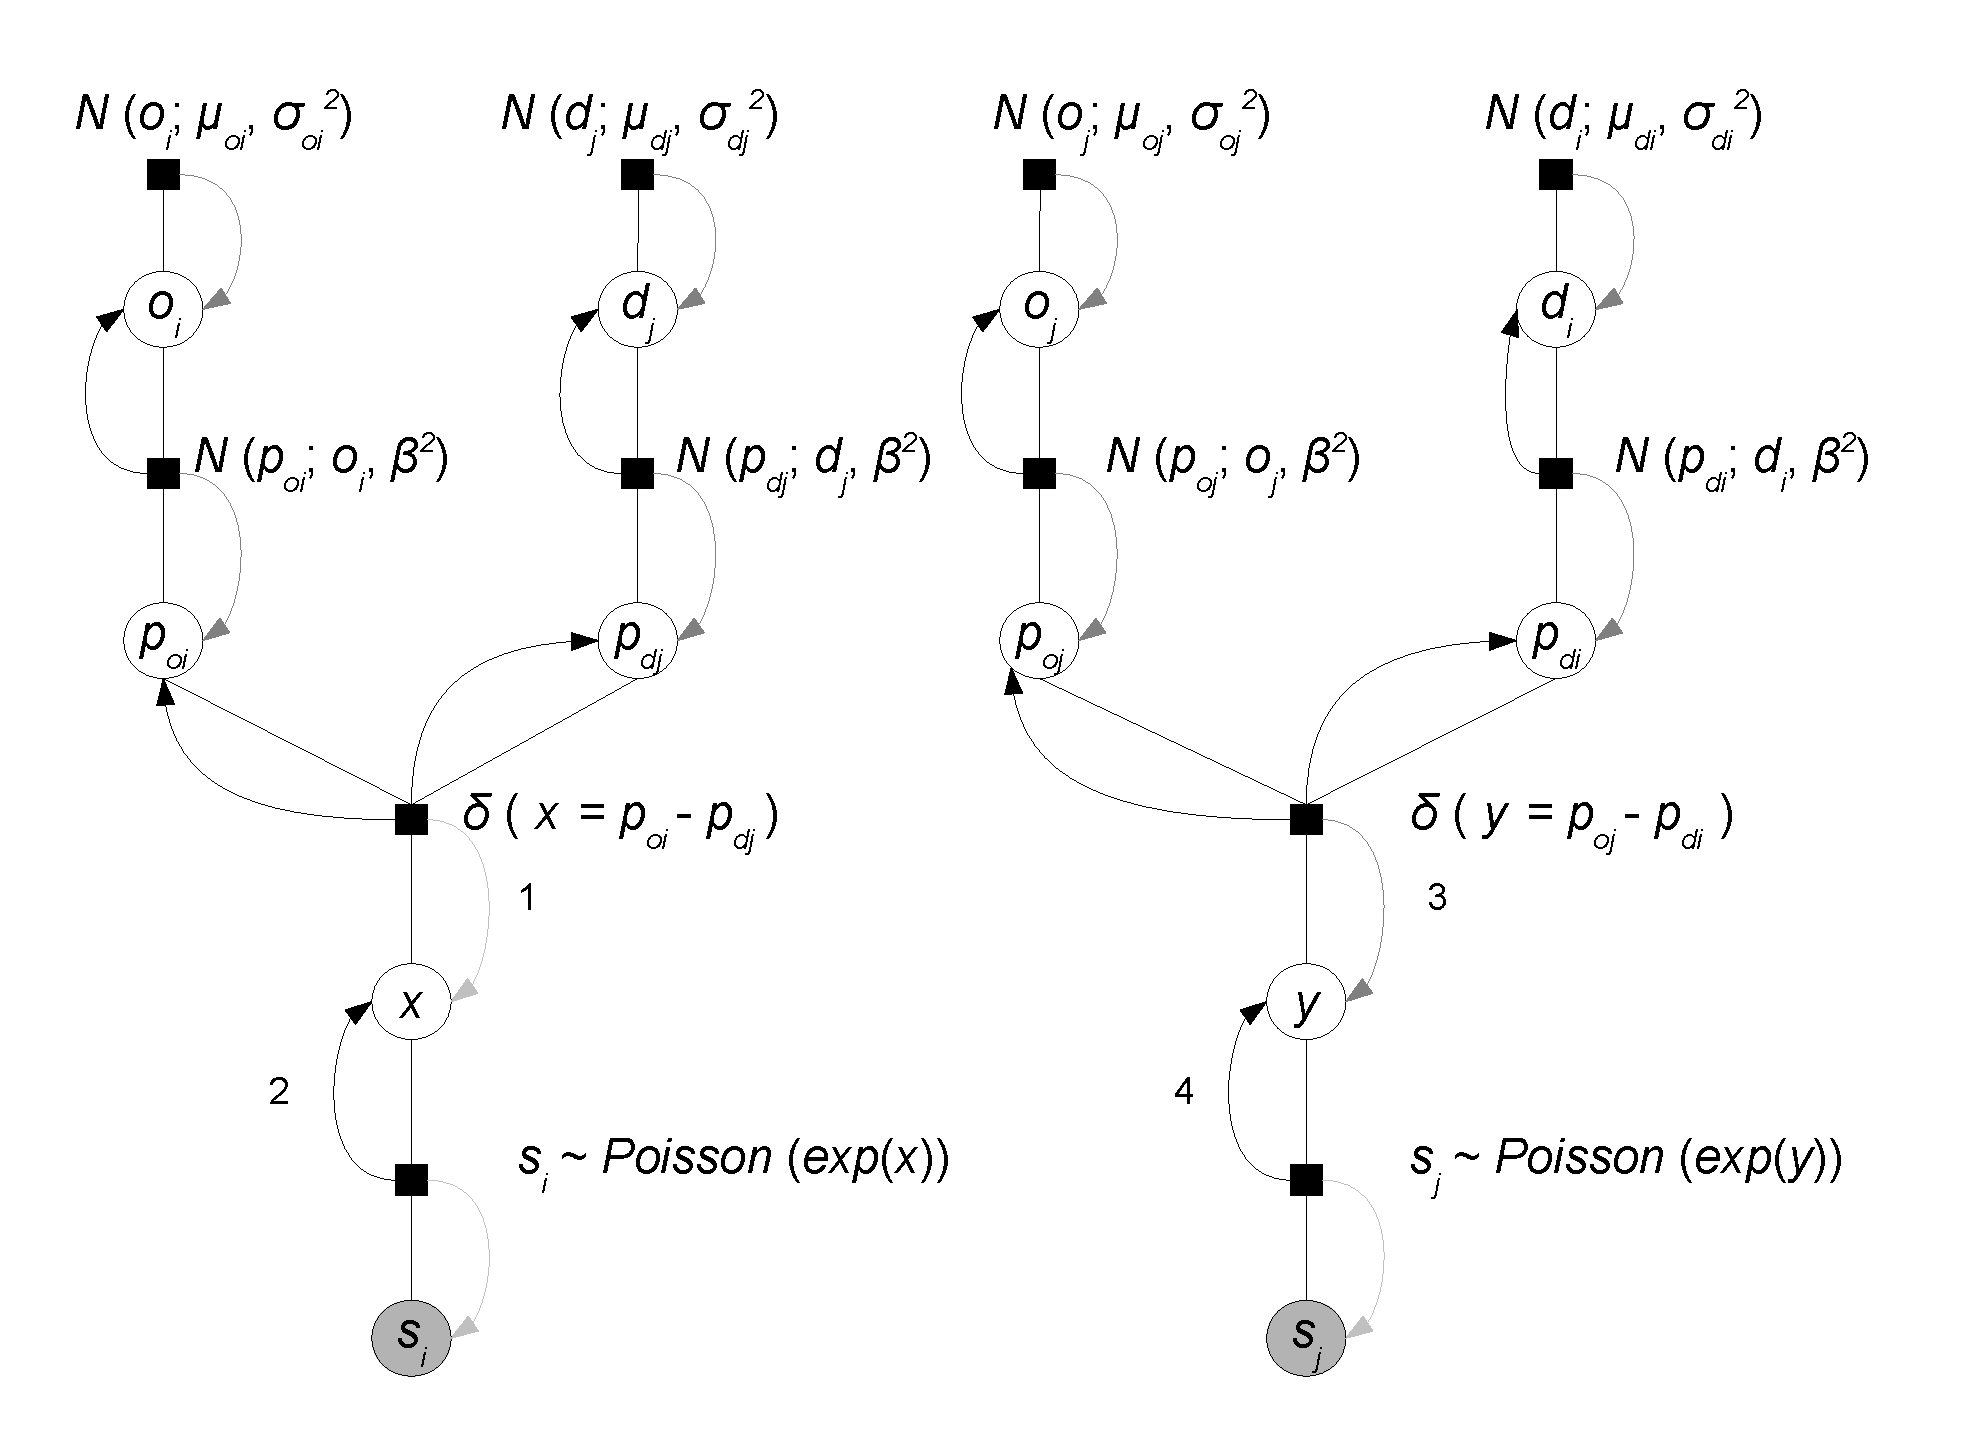
\includegraphics[scale=0.35]{modelAndInference}}
\caption{
The Poisson-OD variants of TrueSkill factor graph for skill update of two teams based on the match score outcome (Left: modeling $s_i$; Right: modeling $s_j$). Note that the score observation factors use the Poisson distribution for the Poisson-OD model. Shaded nodes are observed variables. For each team $i$, it is characterized by offence skill $o_{i}$ (the offence skill of team $i$) and defence skill $d_{i}$ (the defence skill of
team $i$). Given $s_j$ for team $j$, the posterior distributions over $(o_i,d_j)$ are inferred via message passing.
}
\label{fig:trueskill_variant}
\end{figure}
%%%%%%%%%%%%%%%%%%%%%%%%%%%%%%%%%%%%%%%%%%%%%%%%%%%%%%%%%%%%%%%

\subsubsection{Gaussian Offence/Defence Skill Model}

An alternative to the previous Poisson model is to
model $s_i \in \mathbb{R}$ and assume it
is generated as $s_{i}\sim \mathcal{N}(\mu, \gamma^2)$,
where $\mu = p_{oi}-p_{dj}$.  One can similarly
model $s_j$ by applying the same strategy when given $\mu = p_{oj} -
p_{di}$.  We note that unlike the Poisson model, $\mu$ can be negative
here so we need not exponentiate it.  While this allows us to directly
model match outcomes that allow negative team scores (c.f., Halo2 as
discussed in Section~\ref{sec:data_sets}), it is problematic for other
match outcomes that only allow non-negative team scores.  One
workaround would be to introduce a truncated Gaussian model to avoid
the problem of assigning non-zero probability to negative scores, but
we avoid this complication in exchange for the simple and exact
updates offered by a purely Gaussian model.

We show the resulting \emph{Gaussian-OD} model in
Figure~\ref{fig:GaussianOD}, which
differs from our proposed Poisson model only in modeling the observed score $s_i$ ($s_j$) for team $i$ ($j$) given the univariate performance difference variable $x$ ($y$). In this model, all messages passed during inference
are Gaussian, allowing for efficient and exact belief updates.


%%%%%%%%%%%%%%%%%%%%%%%%%%%%%%%%%%%%%%%%%%%%%%%%%%%%%%%%%%%%%%
\begin{figure}[t!]
\centerline{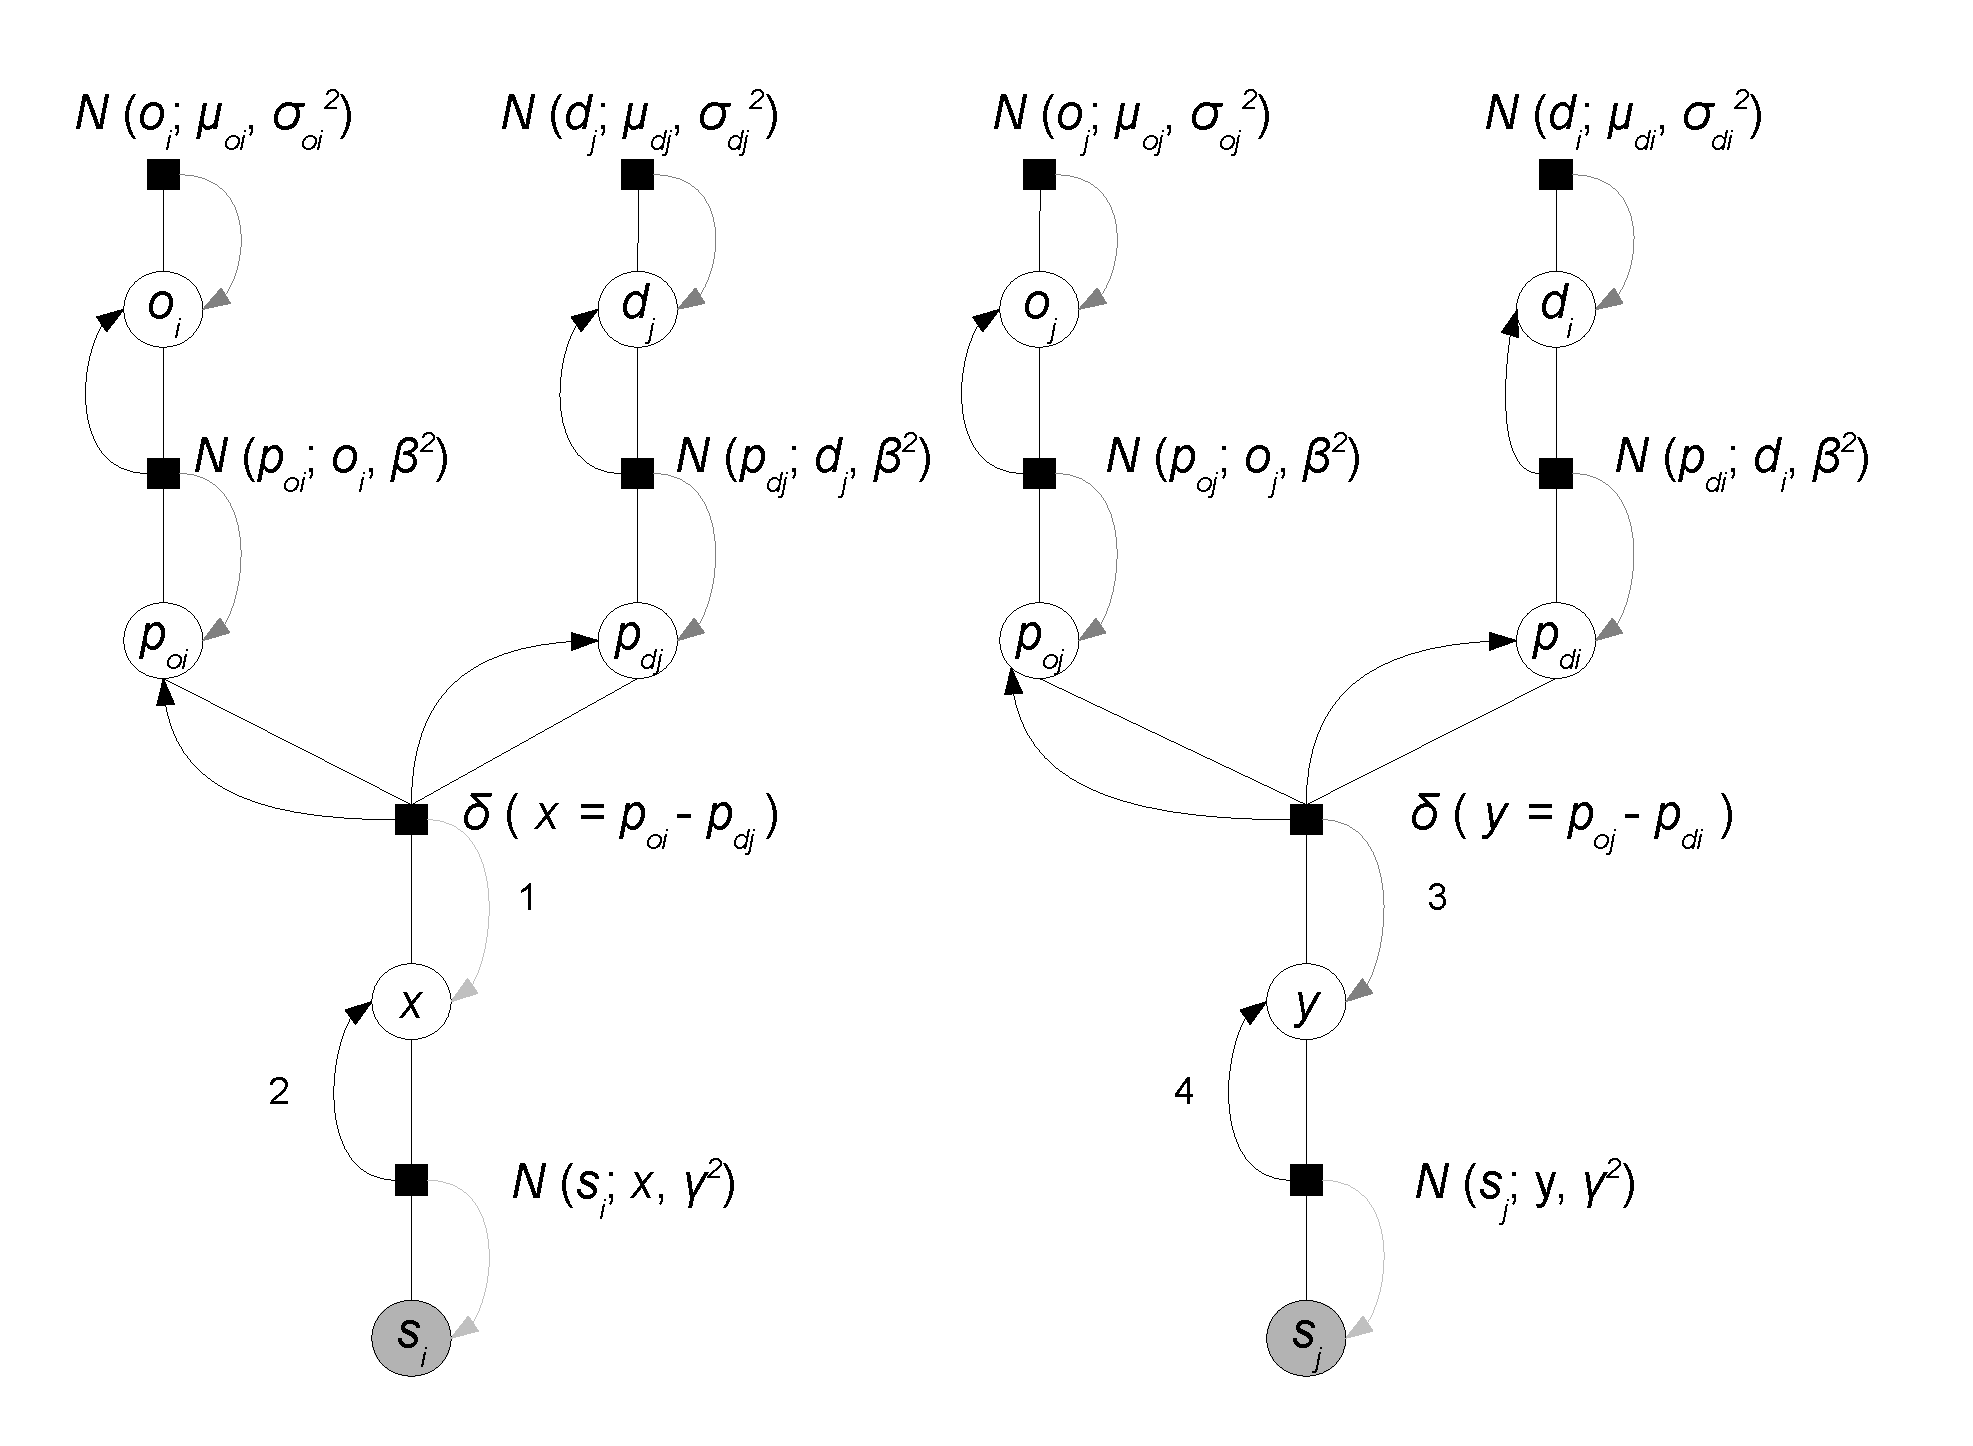
\includegraphics[scale=0.35]{modelAndInferenceGaussianGraphicalModel}}
\caption{
The Gaussian-OD variant of the TrueSkill factor graph for skill update of two teams based on the match score outcome (Left: modeling $s_i$; Right: modeling $s_j$). Note that the score observation factors use the Gaussian distribution for the Gaussian-OD model. Shaded nodes are observed variables. For each team $i$, it is characterized by offence skill $o_{i}$ (the offence skill of team $i$) and defence skill $d_{i}$ (the defence skill of
team $i$). Given $s_j$ for team $j$, the posterior distributions over $(o_i,d_j)$ are inferred via message passing.
}
\label{fig:GaussianOD}
\end{figure}
%%%%%%%%%%%%%%%%%%%%%%%%%%%%%%%%%%%%%%%%%%%%%%%%%%%%%%%%%%%%%%%

\subsection{Gaussian Score Difference (SD) Model}

Again assuming $s_i \in \mathbb{R}$ and $s_j \in \mathbb{R}$,
algebra for the performance means in % the Gaussian offense/defense skill model
Figure~\ref{fig:GaussianOD} gives:
\begin{align}
s_i = p_{oi}-p_{dj}, \qquad \;\; s_j = p_{oj}-p_{di}.
\label{eq:ScoreDifferenceGaussianGraphicalModel}
\end{align}
This implies
\begin{align}
  s_i - s_j &= (p_{oi} - p_{dj}) - (p_{oj} - p_{di})  \nonumber \\
            &= \underbrace{(p_{oi}+p_{di})}_{p_{li}} - \underbrace{(p_{oj}+p_{dj})}_{p_{lj}},
\end{align}
\unindent which is like modeling the score difference with performance
expressions $p_{li}$ and $p_{lj}$ of respective univariate skill levels, $l_i$
and $l_j$.  Motivated by
\eqref{eq:ScoreDifferenceGaussianGraphicalModel}, we propose a score
difference (SD) Gaussian model that uses a likelihood model for the
observed difference $s := s_i - s_j$ specified as $s \sim
\mathcal{N}(p_{li} - p_{lj}, \gamma^2)$ as shown in
Figure~\ref{fig:modelAndInferenceGaussianGraphicalModelScoreDifference}.

%%%%%%%%%%%%%%%%%%%%%%%%%%%%%%%%%%%%%%%%%%%%%%%%%%%%%%%%%%%%%%%%%%%%%
\begin{figure}
\centerline{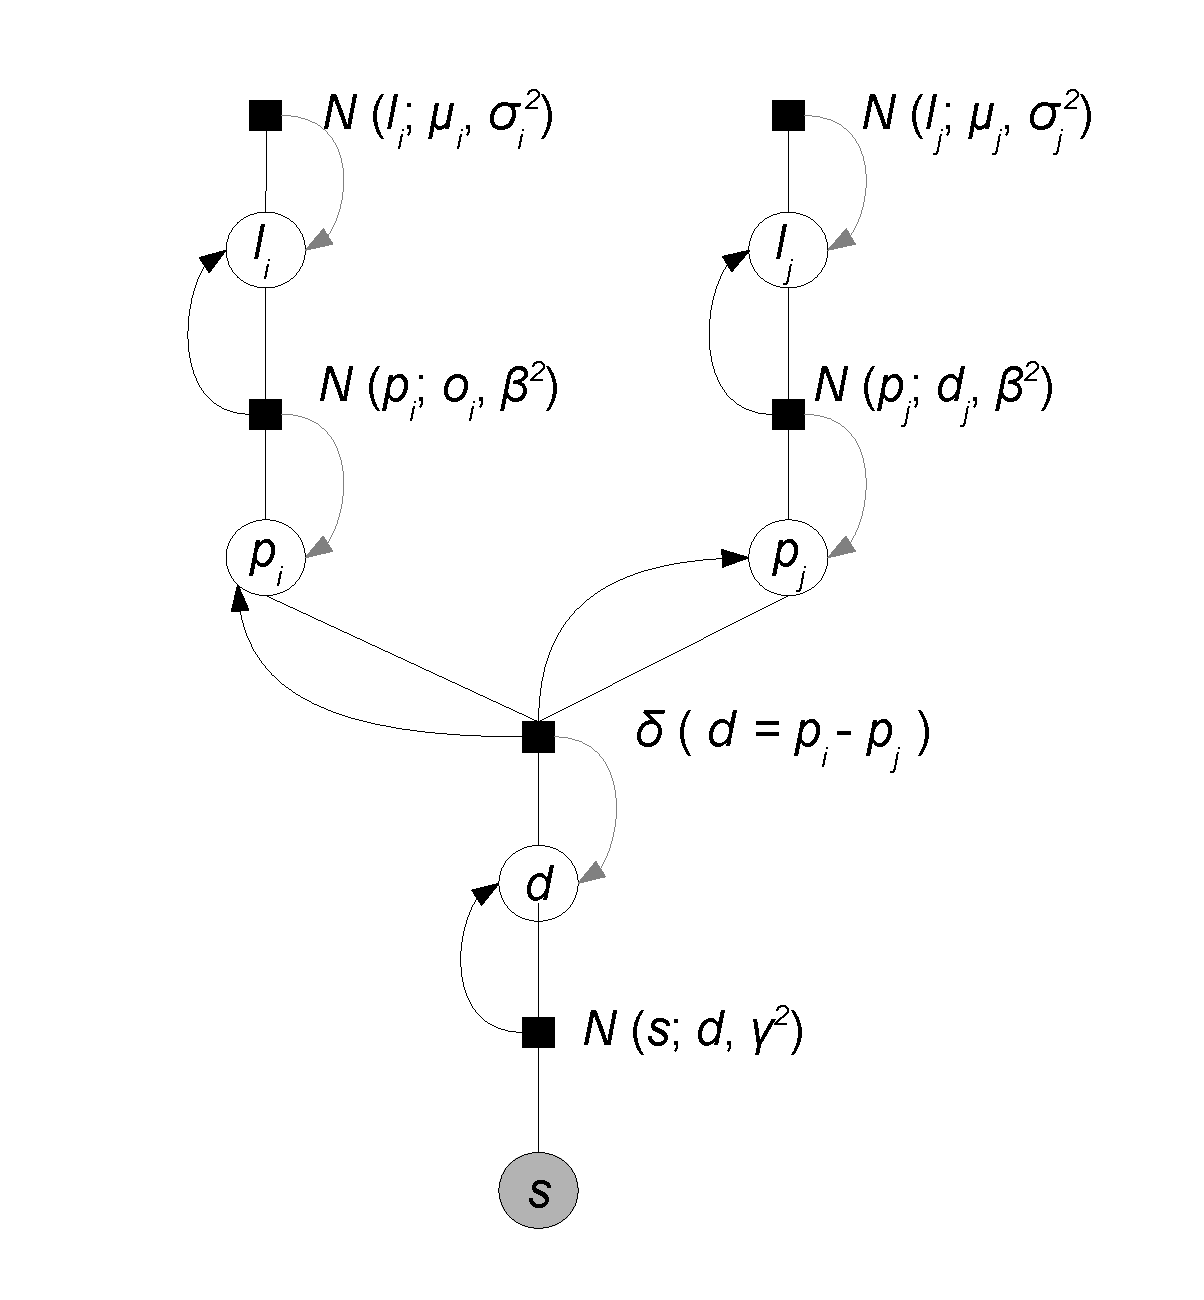
\includegraphics[scale=0.35]{modelAndInferenceGaussianGraphicalModelScoreDifference}}
\caption{\small
The Gaussian-SD variant of the TrueSkill factor graph model for skill update of two teams based on the score difference. Both team
$i$ and team $j$ are characterized by skill level $l_i$ and $l_j$,
respectively. The shaded node $s$ ($s=s_i-s_j$) denotes the score
difference between $s_i$ and $s_j$. Bayesian inference for the posterior
skill level distributions has a closed-form solution.}
\label{fig:modelAndInferenceGaussianGraphicalModelScoreDifference}
\end{figure}
%%%%%%%%%%%%%%%%%%%%%%%%%%%%%%%%%%%%%%%%%%%%%%%%%%%%%%%%%%%%%%%%%%%%%
